\section{Architecture (e.g., back-/frontend)}
This is a CLI application so our frontend is reduced to a simple user interaction on the console. The application itself is built according to the MVC pattern.
\begin{itemize}
    \item \textbf{M}odel: all data interaction (for this application only runtime data) are handled in a model structure
    \item \textbf{V}iew: the user interactions and information displaying are handled in a seperate view
    \item \textbf{C}ontroller: the logic of the application is handled in the controller and some static helper classes
\end{itemize}
The advantage of this pattern is the clear separation of the view, logic and data. With this pattern it is easy to add a graphical interface (a new view). The controller and data models do not need to be changed in this case. The same is the case if something in the data models change.
For persistent storing of data the applications writes local json-files (e.g. configuration). Because this application doesn't need to store a lot of data persistently, it doesn't need a database.
The application is dependent on online archiving services (at the moment archive.today and WayBackMachine). 
The architecture of the application is shown below as an UML class diagram.
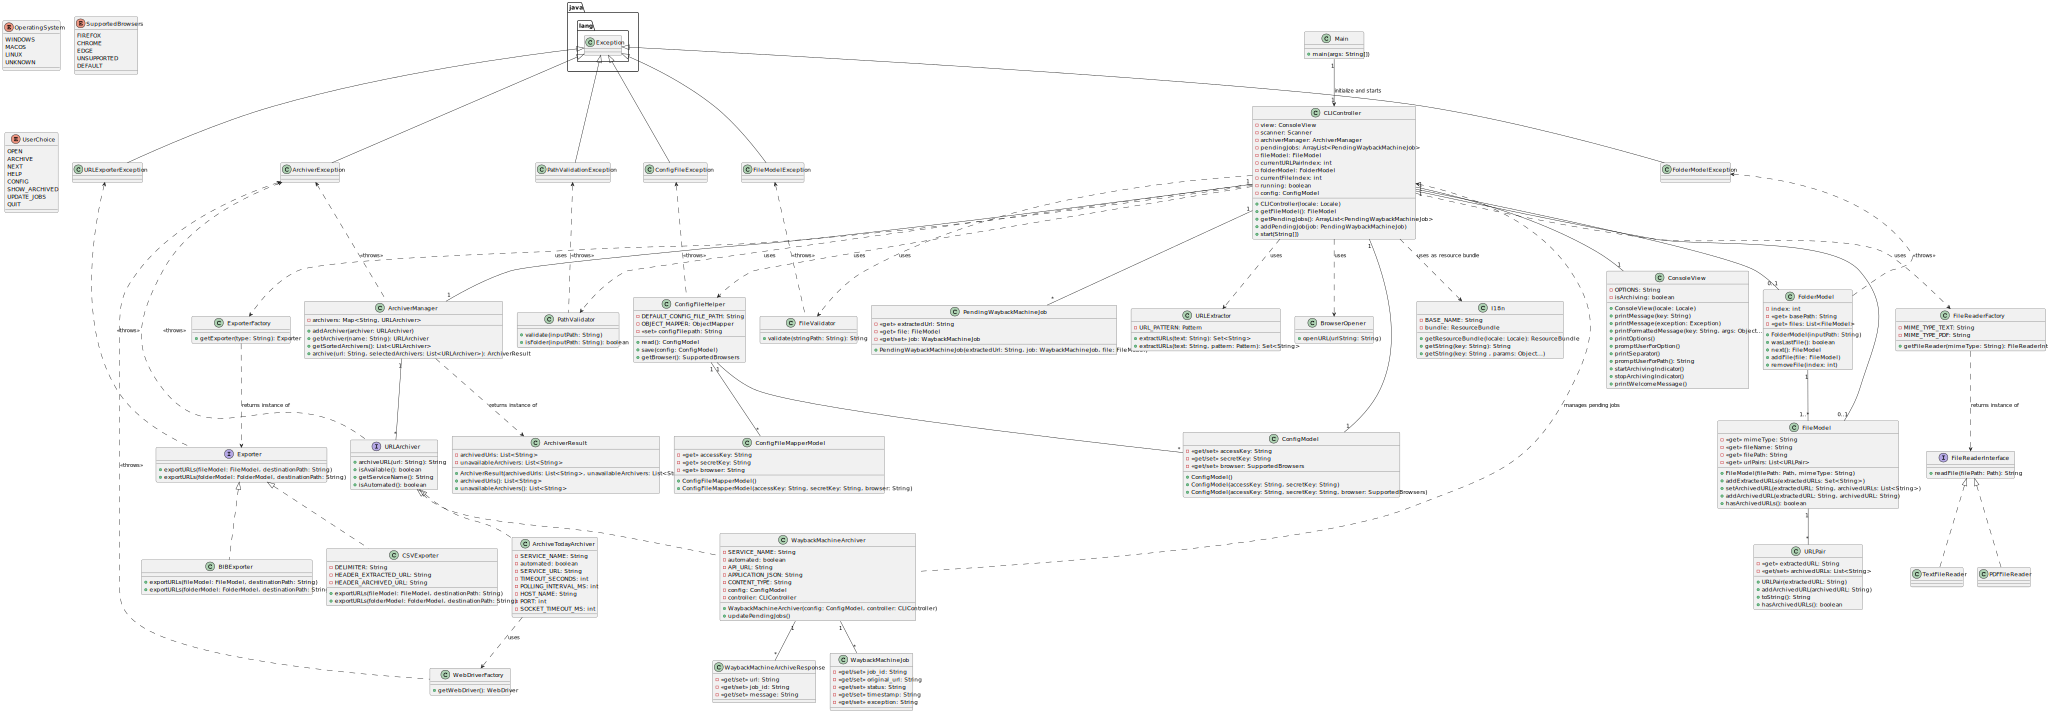
\includepdf[pages=1,fitpaper]{diagrams/uml_diagram.pdf}